\documentclass[12pt]{article}
\usepackage[letterpaper, margin=1in]{geometry}

% \usepackage[dvipsnames]{xcolor}
% \usepackage{xcolor}

\usepackage{graphicx}
\usepackage{subcaption}
\graphicspath{{./figures/}}

\usepackage{hyperref}
\hypersetup{
    colorlinks=true,   
    urlcolor=blue,
}

\usepackage{parskip}
\usepackage{amsmath}
\usepackage{titlesec}

% \usepackage{listings}
\usepackage[numbered, framed]{matlab-prettifier}
\usepackage[ruled,lined,linesnumbered]{algorithm2e}

\usepackage{tikzscale}
\usepackage{pgfplots}
\usepackage{pgfplotstable}
\pgfplotsset{
    compat = newest,
    % width=5cm,
    % height=4cm,
}

\titleformat*{\section}{\large\bfseries}
%\allowdisplaybreaks

% remove vertical spacing above top figure
\makeatletter
\setlength{\@fptop}{0pt}
\makeatother
%

% \renewcommand{\thesubsection}{\thesection.\alph{subsection}}

\title{COMPENG 3SK3 Project 3 Report}
\author{
    Raeed Hassan \\
    hassam41 \\
}

\begin{document}

\maketitle
\clearpage

\section*{Linear Interpolation}
A linear regression based demosaicing algorithm was not implemented for this project, instead this report will demonstrate a linear interpolation algorithm that will use the surrounding pixels to interpolate the red, green, and blue colour components of each pixel based on the surrounding pixels. Depending on the Bayer Pattern applied, the interpolation algorithm will determine which of the surrounding pixels can be used to calculate the three colour components on the pixel. For example, when the Bayer Pattern applied is 'RGGB' and the selected pixel is red, the algorithm will use the pixel's to determine the red component of the image, the average of the pixels on each cardinal direction to determine the green component of the image, and the average of the pixels on each diagonal to determine the blue component of the image. The algorithm does not handle the edges of the image to simplify the coding of the problem.

\section*{MATLAB Implementation}
The code for the MATLAB implementation of this linear interpolation algorithim is implemented in \texttt{project3.m}. The functions implementing linear interpolation are found in \texttt{demosaic\_interpolation.m}. The interpolation algorithm for a 'RGGB' pattern is shown in Listing~\ref{list:rggb}.

\begin{lstlisting}[style=Matlab-editor, caption={MATLAB Implementation of RGGB Interpolation Algorithm}, label={list:rggb}]
function out_img = demosaic_rggb(mosaic_img)
    % Get the size of the input image
    [height, width] = size(mosaic_img);
    
    % Create an output RGB image
    out_img = zeros(height, width, 3);

    mosaic_img = double(mosaic_img);
    
    % Loop over each pixel in the mosaic image
    for i = 1:height-1
        for j = 1:width-1
            % Determine the color of the current pixel based on its position in the pattern
            c1 = mod(i, 2);  % 1 = Red, 2 = Green, 3 = Blue
            c2 = mod(j, 2);

            if (i == 1) || (j == 1)
                continue
            end
            
            % Interpolate the missing color channels based on surrounding pixels
            if c1 == 1 && c2 == 1  % Red
                out_img(i, j, 1) = mosaic_img(i, j);
                out_img(i, j, 2) = (mosaic_img(i, j-1) + mosaic_img(i, j+1) + mosaic_img(i-1, j) + mosaic_img(i+1, j))/4;
                out_img(i, j, 3) = (mosaic_img(i-1, j-1) + mosaic_img(i+1, j-1) + mosaic_img(i-1, j+1) + mosaic_img(i+1, j+1))/4;
            elseif c1 == 0 && c2 == 1  % Green 1
                out_img(i, j, 1) = (mosaic_img(i+1, j) + mosaic_img(i-1, j))/2;
                out_img(i, j, 2) = mosaic_img(i, j);
                out_img(i, j, 3) = (mosaic_img(i, j-1) + mosaic_img(i, j+1))/2;
            elseif c1 == 1 && c2 == 0  % Green 2
                out_img(i, j, 1) = (mosaic_img(i, j-1) + mosaic_img(i, j+1))/2;
                out_img(i, j, 2) = mosaic_img(i, j);
                out_img(i, j, 3) = (mosaic_img(i-1, j) + mosaic_img(i+1, j))/2;
            else  % Blue
                out_img(i, j, 1) = (mosaic_img(i-1, j-1) + mosaic_img(i+1, j-1) + mosaic_img(i-1, j+1) + mosaic_img(i+1, j+1))/4;
                out_img(i, j, 2) = (mosaic_img(i, j-1) + mosaic_img(i, j+1) + mosaic_img(i-1, j) + mosaic_img(i+1, j))/4;
                out_img(i, j, 3) = mosaic_img(i, j);
            end
        end
    end

    out_img = uint8(out_img);
end
\end{lstlisting}

\section*{Visual Comparison}
A visual comparison of \texttt{test1.png} can be seen in Figure~\ref{fig:test1}. We can compare the MATLAB \texttt{demosaic} algorithm in Figure~\ref{fig:test1_matlab} and the linear interpolation algorithm in Figure~\ref{fig:test1_interp}. We can observe that these two algorithms have similar performance, displaying similar colours and showing the same artifacts around edges where there are large changes in colour in the image.

A comparison of \texttt{test2.png} can also be seen in Figure~\ref{fig:test2}. We similarly observe a similar performance between the MATLAB implementation of \texttt{demosaic} and the linear interpolation algorithm.

\section*{Drawbacks of Linear Interpolation}
The linear interpolation demosaicing algorithm results in Figures~\ref{fig:test1_interp} and \ref{fig:test2_interp} demonstrate the flaws and drawbacks of such an interpolation algorithm. Due to the lack of information available for making an interpolation for any given pixel, we can observe that when there should be a large shift in colour between pixels it will often resulting in artifacting around edges of objects in the scene. This artifacting can also result in the image appearing more blocky than it should given its resolution.

One potential way to tackle the drawbacks of such an approach is to simply increase the amount of information available to the algorithm. For example, if each pixel accounted for the next several pixels around it when performing the interpolation, it would likely handle edges of objects better. Similarly, a linear regression algorithm that solves the linear least square problem could appropriately assign weights to each surrounding pixels contribution to more accurately calculate a missing colour component past simply taking the average.

\begin{figure}[htp]
    \centering
    \begin{subfigure}[b]{0.53\textwidth}
        \centering
        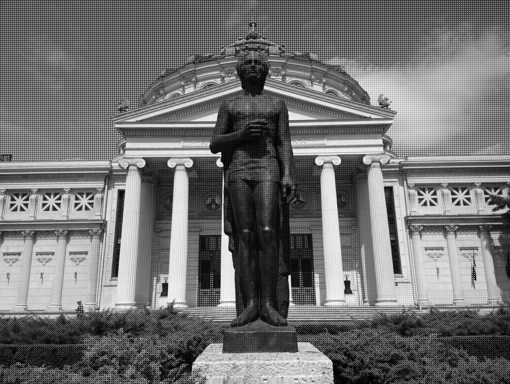
\includegraphics[width=\textwidth]{test1}
        \caption{Test Image}
        \label{fig:test1_mosaic}
    \end{subfigure}
    \hfill
    \begin{subfigure}[b]{0.53\textwidth}
        \centering
        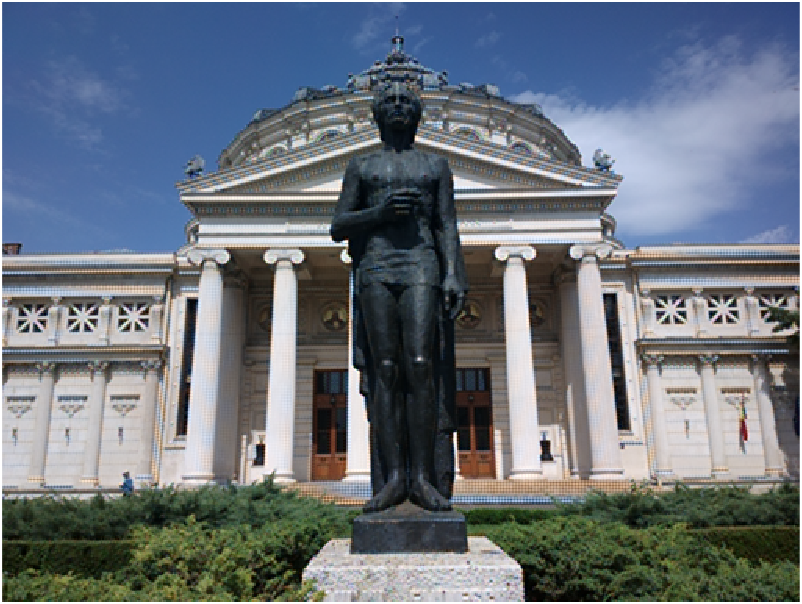
\includegraphics[width=\textwidth]{test1_matlab}
        \caption{MATLAB \texttt{demosaic} Output}
        \label{fig:test1_matlab}
    \end{subfigure}
    \hfill
    \begin{subfigure}[b]{0.53\textwidth}
        \centering
        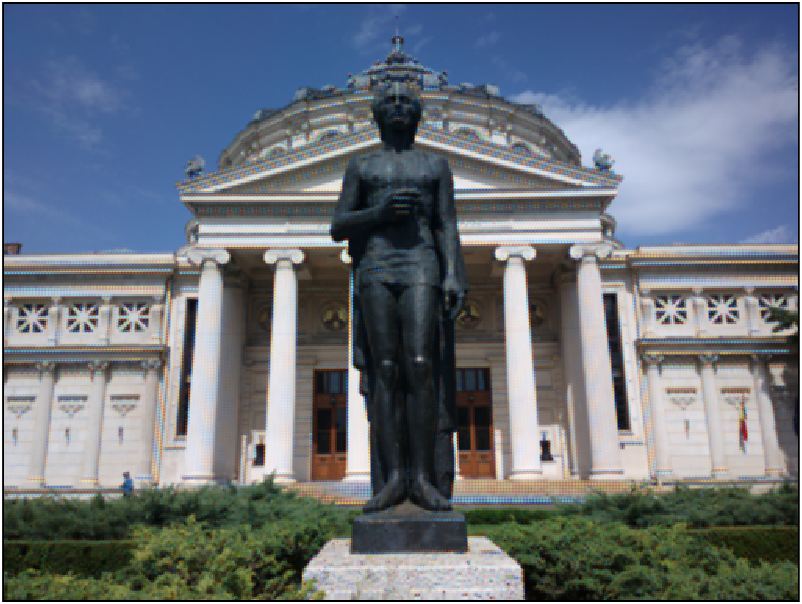
\includegraphics[width=\textwidth]{test1_interp}
        \caption{Linear Interpolation Demosaicing Output}
        \label{fig:test1_interp}
    \end{subfigure}
       \caption{Test Image \texttt{test1.png}}
       \label{fig:test1}
\end{figure}

\begin{figure}[htp]
    \centering
    \begin{subfigure}[b]{0.6\textwidth}
        \centering
        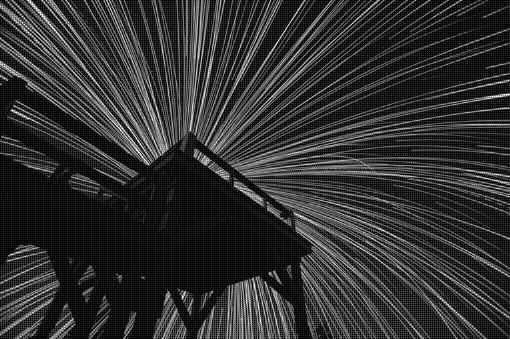
\includegraphics[width=\textwidth]{test2}
        \caption{Test Image}
        \label{fig:test2_mosaic}
    \end{subfigure}
    \hfill
    \begin{subfigure}[b]{0.6\textwidth}
        \centering
        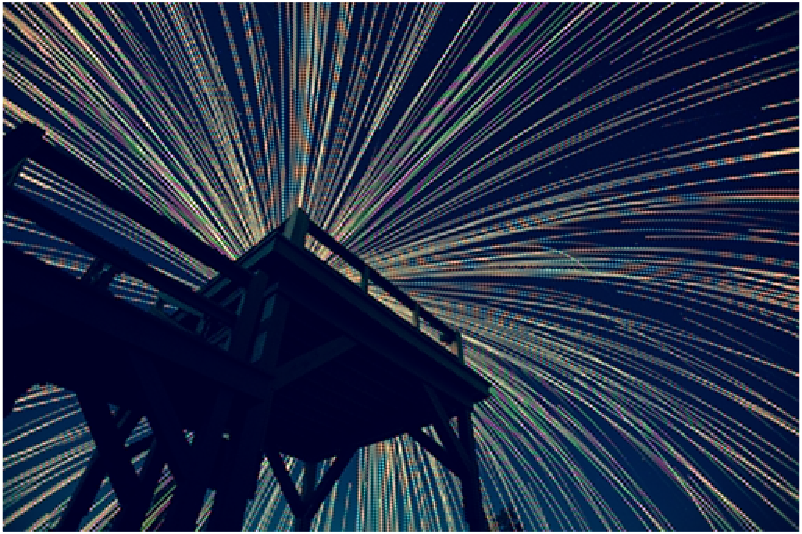
\includegraphics[width=\textwidth]{test2_matlab}
        \caption{MATLAB \texttt{demosaic} Output}
        \label{fig:test2_matlab}
    \end{subfigure}
    \hfill
    \begin{subfigure}[b]{0.6\textwidth}
        \centering
        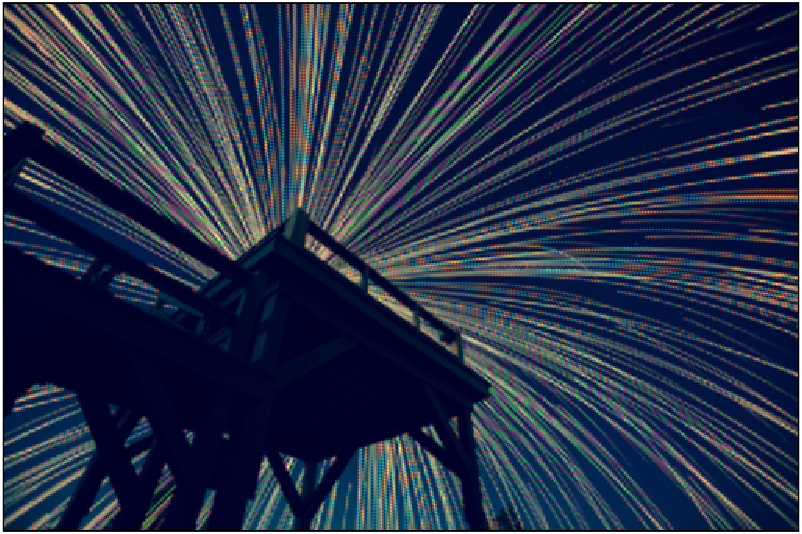
\includegraphics[width=\textwidth]{test2_interp}
        \caption{Linear Interpolation Demosaicing Output}
        \label{fig:test2_interp}
    \end{subfigure}
       \caption{Test Image \texttt{test2.png}}
       \label{fig:test2}
\end{figure}

% The quality of the estimated coordinates of markers was evaluated by computing the RSME between the estimated coordinates and the ground-truth markers with the formula below:

% \begin{equation}
%     \text{RSME} = \sqrt{\frac{1}{N} \sum_{i=1}^{N} \lVert \mathbf{\tilde{p}}_\text{i} - \mathbf{p}_\text{i} \rVert_2^2} 
% \end{equation}

% The RSME was calculated in MATLAB with the function shown in Listing~\ref{list:rsme}.

% \begin{lstlisting}[style=Matlab-editor, caption={MATLAB Implementation of RSME}, label={list:rsme}]
% function val = RSME(p_est, N)
%     % load ground-truth oordinates, (pts_marks_gt)
%     load('data for student/gt_R5_L40_N100_K21.mat','pts_marks_gt');

%     val = sqrt((1/N) * norm(p_est - pts_marks_gt)^2);
% end
% \end{lstlisting}

% \subsection*{Fine-tune $\lambda$}
% To determine the optimal $\lambda$, $\lambda_{op}$, we change the value of $\lambda$ when $\mathbf{p}^{(0)}$ is the average of the $K$ measured coordinates to reduce the RMSE after 50 iterations of Newton's method. We observe that lower value of $\lambda$ is, the lower the converged RSME is. We select $\lambda = 10^{-4}$ as $\lambda_{op}$ as continuing to decrease $\lambda$ any further results in a negligible reduction in the RSME. Figure~\ref{fig:lambda} plots the curve of the converged RMSE against $\lambda$. 

% \begin{filecontents}[overwrite]{./figures/lambda.tikz}
% \begin{tikzpicture}
%     \begin{axis}[
%         % title = {RSME vs. $\lambda$},
%         width = \textwidth,
%         %height = 150,
%         xmin = 0.01, xmax = 100,
%         xmode = log,
%         % ymin = 0, ymax = 0.04,
%         ylabel = Real Mean Square Error (RSME), xlabel = $\lambda$ relative to $\lambda_{op}$,
%         yticklabel style={
%             /pgf/number format/fixed,
%             /pgf/number format/precision=5
%         },
%         scaled y ticks=false,
%         xticklabel style={
%             /pgf/number format/fixed,
%             /pgf/number format/precision=3
%         },
%         scaled x ticks=false,
%         legend pos = north east,
%     ]

%     \addplot table [y=rsme, x=lambda] {./data/lambda.dat};
%     \end{axis}
% \end{tikzpicture}
% \end{filecontents}

% \subsection*{Fine-tune the initialization $\mathbf{p}^{(0)}$}

% The curves of RSME against iterations given three different initialization schemes at $\lambda = \lambda_{op} = 10^{-4}$ are shown below. Figure~\ref{fig:rsme_mean} shows the RSME against iterations given $\mathbf{p}^{(0)}$ is the average of the $K$ measured coordinates. Figure~\ref{fig:rsme_first} shows the RSME against iterations given $\mathbf{p}^{(0)}$ is the first measured coordinate. Figure~\ref{fig:rsme_randn} shows the RSME against iterations given $\mathbf{p}^{(0)}$ is a normally distributed random vector.

% The number of iterations needed varies depending on the chosen initialization scheme. When $\mathbf{p}^{(0)}$ is the average of the $K$ measured coordinates, we observe the initial error (RSME) to be relatively close to the converged value, and quickly converges within 20 iterations. When selecting the first measured coordinate instead, we see more iterations are needed to converge and initial error is larger (nearly an order of magnitude larger), but the final converged error is similar. Similarly, when switching to a normally distributed random vector for the initialization scheme we observe the number of iterations needed for convergence and the initial error both increase significantly (again increasing by an order of magnitude from the previous scheme), while the final converged error is similar.

% We can conclude that the converged RSME will be similar regardless of the initialization scheme used, however the number of iterations required for convergence and the initial RSME will vary depending on the scheme.

% \begin{figure}[htp]
%     \centering
%     \caption{RSME against $\lambda$}
%     \label{fig:lambda}
%     \includegraphics[width=\textwidth]{lambda.tikz}
% \end{figure}

% \begin{filecontents}[overwrite]{./figures/rsme_mean.tikz}
% \begin{tikzpicture}
%     \begin{axis}[
%         title = {RSME vs. Number of Iterations},
%         width = \textwidth,
%         %height = 150,
%         xmin = 0, xmax = 100,
%         ymin = 0, ymax = 0.04,
%         ylabel = Real Mean Square Error (RSME), xlabel = Number of Iterations,
%         yticklabel style={
%         /pgf/number format/fixed,
%         /pgf/number format/precision=3
%         },
%         scaled y ticks=false,
%         legend pos = north east,
%     ]

%     \addplot table [y=rsme_mean, x=max_iterations] {./data/rsme.dat};
%     \end{axis}
% \end{tikzpicture}
% \end{filecontents}

% \begin{filecontents}[overwrite]{./figures/rsme_first.tikz}
% \begin{tikzpicture}
%     \begin{axis}[
%         title = {RSME vs. Number of Iterations},
%         width = \textwidth,
%         %height = 150,
%         xmin = 0, xmax = 100,
%         ymin = 0, ymax = 0.25,
%         ylabel = Real Mean Square Error (RSME), xlabel = Number of Iterations,
%         yticklabel style={
%         /pgf/number format/fixed,
%         /pgf/number format/precision=3
%         },
%         scaled x ticks=false,
%         legend pos = north east,
%     ]

%     \addplot table [y=rsme_first, x=max_iterations] {./data/rsme.dat};
%     % \addlegendentry{Choose First Measured Coordinates}

%     \end{axis}
% \end{tikzpicture}
% \end{filecontents}

% \begin{filecontents}[overwrite]{./figures/rsme_randn.tikz}
% \begin{tikzpicture}
%     \begin{axis}[
%         title = {RSME vs. Number of Iterations},
%         width = \textwidth,
%         %height = 150,
%         xmin = 0, xmax = 100,
%         ymin = 0, ymax = 25,
%         ylabel = Real Mean Square Error (RSME), xlabel = Number of Iterations,
%         yticklabel style={
%         /pgf/number format/fixed,
%         /pgf/number format/precision=3
%         },
%         scaled x ticks=false,
%         legend pos = north east,
%     ]

%     \addplot table [y=rsme_randn, x=max_iterations] {./data/rsme.dat};
%     % \addlegendentry{Set as Normally Distributed Random Vector}

%     \end{axis}
% \end{tikzpicture}
% \end{filecontents}

% \begin{figure}[htp]
%     \centering
%     \caption{RSME against Iterations for Different Initialization Schemes}
%     \begin{subfigure}[b]{0.62\textwidth}
%         \caption{RSME for Average of Measured Coordinates}
%         \label{fig:rsme_mean}
%         \includegraphics[width=\textwidth]{rsme_mean.tikz}
%     \end{subfigure}
%     \begin{subfigure}[b]{0.62\textwidth}
%         \caption{RSME for First of Measured Coordinates}
%         \label{fig:rsme_first}
%         \includegraphics[width=\textwidth]{rsme_first.tikz}
%     \end{subfigure}
%     \begin{subfigure}[b]{0.62\textwidth}
%         \caption{RSME for Normally Distributed Random Vector}
%         \label{fig:rsme_randn}
%         \includegraphics[width=\textwidth]{rsme_randn.tikz}
%     \end{subfigure}
% \end{figure}

% \begin{figure}[htp]
%     \centering
%     \caption{RSME for Average of Measured Coordinates}
%     \label{fig:rsme_mean}
%     \includegraphics[width=\textwidth]{rsme_mean.tikz}
% \end{figure}

% \begin{figure}[htp]
%     \centering
%     \caption{RSME for First of Measured Coordinates}
%     \label{fig:rsme_first}
%     \includegraphics[width=\textwidth]{rsme_first.tikz}
% \end{figure}

% \begin{figure}[htp]
%     \centering
%     \caption{RSME for Normally Distributed Random Vector}
%     \label{fig:rsme_randn}
%     \includegraphics[width=\textwidth]{rsme_randn.tikz}
% \end{figure}

\end{document}